\documentclass[10pt]{article}
\usepackage[utf8]{vietnam}
\usepackage{fontspec}      % font selection
%\setmainfont{Cambria}
\setmainfont{Times New Roman}
\usepackage{breqn}         % automatic equation breaking
\usepackage{microtype}     % microtypography, reduces hyphenation
\usepackage{polyglossia}   % language selection
\setmainlanguage{vietnamese}

\usepackage{graphicx}      % graphics support

\usepackage[font=small,labelformat=simple,]{caption}   % customizing captions

\usepackage{titlesec}      % customizing section titles
\titleformat{\section}{\itshape\large}{}{0em}{}
\titlespacing{\section}{0pt}{8pt}{4pt}
\titleformat{\subsection}{\itshape}{}{0em}{}
\titlespacing{\subsection}{0pt}{4pt}{2pt}
\titleformat{\subsubsection}[runin]{\bf\scshape}{}{0em}{}
\titlespacing{\subsubsection}{0pt}{5pt}{5pt}

\usepackage[papersize={3.6in,4.8in},hmargin=0.1in,vmargin={0.1in,0.1in}]{geometry}  % page geometry

\usepackage{fancyhdr}   % headers and footers
\pagestyle{fancy}
\fancyhead{}            % clear page header
\fancyfoot{}            % clear page footer

\setlength{\abovecaptionskip}{2pt} % space above captions
\setlength{\belowcaptionskip}{0pt} % space below captions
\setlength{\textfloatsep}{2pt}     % space between last top float or first bottom float and the text
\setlength{\floatsep}{2pt}         % space left between floats
\setlength{\intextsep}{2pt}        % space left on top and bottom of an in-text float

\begin{document}

    In another moment down went Alice after it, never once considering how in the world she was to get out again.
    Trong một thoáng chốc suy nghĩ sau khi Alice quyết định đuổi theo nó, mà không suy nghĩ đến việc làm thế quái nào mà cô ấy có thể thoát ra sau đó được.

    \section{Wonderful section title}

    Either the well was very deep, or she fell very slowly, for she had plenty of time as she went down to look
    \begin{figure}[htb]
        \centering
        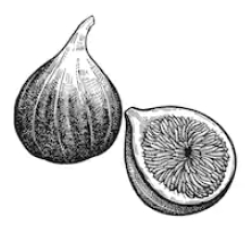
\includegraphics[width=0.5 \textwidth]{fig1}
        \caption{Quite wide picture, resized to fit}
    \end{figure}
    about her and to wonder what was going to happen next.

    \subsection{Tufte-style subsection}

    then she looked at the sides of the well

    \subsubsection{Saving space running in} and noticed that they were filled with cupboards and book\-shel\-ves.

    \begin{dmath}[label={sna74}]
        \frac{1}{6} \left(\sigma(k,h,0) +\frac{3(h-1)}{h}\right)
        +\frac{1}{6} \left(\sigma(h,k,0) +\frac{3(k-1)}{k}\right)
        =\frac{1}{6} \left(\frac{h}{k} +\frac{k}{h} +\frac{1}{hk}\right)
        +\frac{1}{2} -\frac{1}{2h} -\frac{1}{2k},
    \end{dmath}

\end{document}